
\documentclass[11pt,reqno]{amsart} % use larger type; default would be 10pt

\usepackage{multicol}
\usepackage{my_packages}
\usepackage{tikz_packages}
\usepackage{float}
\tdplotsetmaincoords{60}{125} % view angle in spherical coordinates
\renewcommand{\thesection}{\Roman{section}} 
\renewcommand{\thesubsection}{\thesection.\Roman{subsection}}

\title{Spacecraft Trajectory Design near Asteroid 4769 Castalia}
\author{Shankar Kulumani}
\thanks{PhD Candidate, Department of Mechanical and Aerospace Engineering, Email:~\href{mailto:sklumani@gwu.edu}{skulumani@gwu.edu}}

\author{Taeyoung Lee}
\thanks{Assistant Professor, Department of Mechanical and Aerospace Engineering, Email:~\href{mailto:tylee@gwu.edu}{tylee@gwu.edu}}

\date{} % Activate to display a given date or no date (if empty),
         % otherwise the current date is printed 

\begin{document}
\maketitle
\begin{multicols}{2}
\section{Introduction}
% Motivation for missions/studying asteroids
Small solar system bodies, such as asteroids and comets, are of significant interest to the scientific community; These small bodies offer great insight into the early formation of the solar system.
This insight offers additional detail into the formation of the Earth and also the probable formation of other planetary bodies.
Of particular interest are those near-Earth asteroids (NEA) which inhabit heliocentric orbits in the vicinity of the Earth.
These easily accessible bodies provide attractive targets to support space industrialization, mining operations, and scientific missions.
NEAs potentially contain many materials such as those useful for propulsion, construction, or for use in semiconductors.
Also, many bodies contain highly profitable materials, such as precious or strategic metals~\cite{ross2001}.
In addition, these NEAs are also of concern for their potential to impact the Earth.
Asteroids and comets are the greatest threat to future civilizations and as a result there is a focused effort to mitigate these risks~\cite{wie2008}.
In spite of the great interest in asteroids, the operation of spacecraft in their vicinity is a challenging problem.

% Difficulty in system model
While there has been significant study of interplanetary transfer trajectories, relatively less analysis has been conducted on operations in the vicinity of asteroids.
The dynamic environment around asteroids is strongly perturbed and challenging for analysis and mission operation.
Due to their low mass, which results in a low gravitational attraction, asteroids may have irregular shapes and potentially chaotic spin states.
Furthermore, since the magnitude of the gravitational attraction is relatively small, non-gravitational effects, such as solar radiation pressure or third-body effects, become much more significant.
As a result, the orbital environment is generally quite complex and it is difficult to generate analytical insights.

\subsection{Research Question}
In this paper, we extend the design method previously developed in the three-body problem to motion about asteroids.
The authors present a systematic method of generating optimal transfer orbits about asteroids.
Our systematic approach avoids the difficulties in selecting an appropriate initial guess for optimization.
We instead utilize the concept of the reachability set to enable a simple methodology of selecting initial conditions to achieve general orbital transfers.
This method allows us to avoid the difficulties inherent in choosing valid initial conditions for the computation of optimal transfer trajectories.
We develop the optimal control formulation and apply this method to an example transfer about asteroid 4769 Castalia.

\subsection{Motivation}

The potential for asteroid impact presents one of the largest threats to the future of humanity.
Interplanetary space, while relatively empty by human standards, Earth is in a ``cosmic shooting gallery''.
There is a continual bombardment of the Earth by a large range of planetary material, from dust particles to the much less common size of several kilometers or larger.
This was vividly demonstrated in 2013 by the Chelyabinsk air burst, where a \SIrange{10}{20}{\meter} asteroid exploded over the Russian city of Chelyabinsk on  15 February 2013.
This event released the equivalent of approximately \SI{590}{\kilo\tonne} of TNT and is one of the few Earth impacts with eyewitness video footage.
In spite of the meteorite exploding at over \SI{100}{\kilo\meter}, the shock wave was powerful enough to knock people off their feet and caused widespread damage to the surrounding area.

It is only a matter of time before a much more devastating body arrives at the Earth.
As a result, it is imperative to develop spacecraft methodologies to avert any future impact scenarios.
There is a growing body of research investigating a variety of impact mitigation techniques~\cite{wie2008,pitz2014}.
A key requirement of these future missions is the ability to effectively design spacecraft trajectories. 
In addition, a completly new design paradigm is required as the typical methods developed for use around the Earth or other large bodies is not applicable. 

\section{Orbital Transfer Example}
\begin{figure}[H]
\begin{scaletikzpicturetowidth}{0.2\columnwidth}
    \begin{tikzpicture}[tdplot_main_coords,
          poincare/.style={opacity=.2,very thick,fill=blue},
          orbit/.style={very thick,black},
          orbit hidden/.style={very thick,dashed},
          grid/.style={very thin,gray},
          axis/.style={->,blue,thick},
          reachability/.style={thick,blue}, scale=0.6]

        % nodes for the poincare section
        \node[label=above:\(\Sigma\)] (upper_right) at (0,5,5) {};
        \node[] (upper_left) at (0,1,5) {};
        \node[] (lower_left) at (0,1,0) {};
        \node[] (lower_right) at (0,5,0) {};

        % draw poincare section
        \draw[poincare] (upper_right.center) -- (upper_left.center) -- (lower_left.center) -- (lower_right.center) -- (upper_right.center);
        
        % draw a periodic orbit
        \coordinate (center) at (0,0,2);
        \node[label=below:\(\vecbf{x}_0\)] (x0) at (0,3,2) {};
        % \node[label=below:\(\vecbf{x}_n\)] at (x0) {};
        \filldraw (x0) circle (3pt);

        % \tdplotdrawarc[orbit hidden]{(center)}{3}{90}{200}{}{};
        \tdplotdrawarc[orbit,<-]{(center)}{3}{-160}{90}{}{};

        % draw reachability set on the poincare section
        \coordinate (reach) at (0,4.5,2);
        \tdplotsetthetaplanecoords{90}

        \draw[tdplot_rotated_coords,grid] (x0) -- (reach);
        \draw[tdplot_rotated_coords,grid] (x0) -- ++(-45:1.5);

        \tdplotdrawarc[tdplot_rotated_coords,grid]{(x0)}{0.5}{-45}{90}{above}{\(\phi\)};

        % draw terminal state on reachability set
        \node[tdplot_rotated_coords,label=above:\(\vecbf{x}_f\)] (xf) at ($ (x0)+(-45:1.5) $) {};
        \filldraw (xf) circle (3pt);

        \node[tdplot_rotated_coords,label=below:\(J\)] at (xf) {};

        \tdplotdrawarc[tdplot_rotated_coords,reachability]{(x0)}{1.5}{0}{360}{}{};
        % place
    \end{tikzpicture}
\end{scaletikzpicturetowidth}
\caption{Reachability Set\label{fig:reachability_set}}
\end{figure}
We utilize the concept of a reachability set to design our transfer trajectories.
\Cref{fig:reachability_set} illustrates this methodology.
Without any control input, the trajectories will follow the system dynamics, \( \psi(t, \vecbf{x}_0 ) \) and intersect the \Poincare section at \( \vecbf{x}_n\).
The addition of a control input allows the spacecraft to depart from the natural dynamics and intersect the section at another location denoted by the dashed circle.
We use the cost function \( J \) to define a distance metric on the \Poincare section.
Maximization of \( J \), or the minimization of \( -J \), along various directions, which are parameterized using \( \phi_d \), on the \Poincare section allows us to generate the largest reachability set under the bounded control input.
We then select a trajectory from the reachable set which lies closest to the desired target. 
By repeating the calculation we can determine a transfer about asteroid 4769 Castalia.

We present an example transfer of a spacecraft about the asteroid 4769 Castalia.  
We model the thruster of the spacecraft as a generic acceleration vector in the body-fixed asteroid frame. 
The acceleration magnitude is chosen to emulate a physically realizable thruster system, such as those found on many operational ion or hall effect thrusters~\cite{goebel2008,choueiri2009}.
\begin{figure}[H]
    % \centering 
    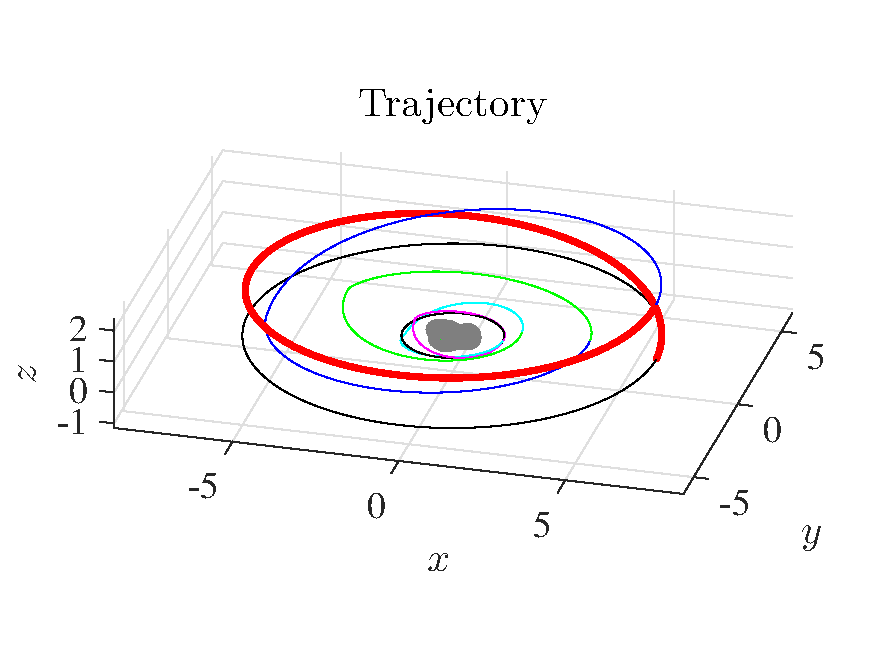
\includegraphics[width=\columnwidth,height=\columnwidth,keepaspectratio]{figures/trajectory_3d.pdf} 
    \caption{Transfer Trajectory}
    \label{fig:transfer_3d} 
\end{figure}

The objective is to transfer the spacecraft between two periodic equatorial orbits about Castalia.
\Cref{fig:transfer_3d} shows the initial, \( \vecbf{x}_i \), and target, \( \vecbf{x}_t\), periodic orbits which lie in the equatorial plane of Castalia.
Our goal is to transfer from a lower altitude to a higher altitude while remaining in the equatorial plane of the asteroid.
This type of scenario would occur frequently during mapping and observation missions to asteroids.

We can see in~\cref{fig:transfer_3d} that this transfer requires four iterations of the reachable set computation. 
Each reachability set progressively approaches the target periodic orbit.
The final computation intersects the target periodic orbit on our chosen \Poincare section and allows for a complete orbital transfer between the periodic orbits. 

\bibliographystyle{amsplain}
\bibliography{library.bib}

\end{multicols}
\end{document}
